\documentclass{beamer}
% \documentclass[handout]{beamer}

\usepackage{amsmath}
\usepackage{beamerthemesplit}
\usepackage{fancybox}
\usepackage{hyperref}
\usepackage{color}
\usepackage{listings}


\makeatletter
\newcommand\code{\bgroup\@makeother\_\@makeother\~\@makeother\$\@codex}
\def\@codex#1{{\normalfont\ttfamily\hyphenchar\font=-1 #1}\egroup}
\makeatother

\newcommand{\bX}{\boldsymbol{X}}
\newcommand{\bx}{\boldsymbol{x}}
\newcommand{\by}{\boldsymbol{y}}
\newcommand{\bbeta}{\boldsymbol{\beta}}
\newcommand{\bepsilon}{\boldsymbol{\epsilon}}
\newcommand{\bs}[1]{\boldsymbol{#1}}


\definecolor{gray}{rgb}{.6,.6,.6}
\definecolor{orange}{rgb}{1,0.5,0}
\definecolor{grayish}{rgb}{.775, .775, .775}
\definecolor{dkgray}{rgb}{.375, .375, .375}
\definecolor{dkgreen}{rgb}{0,0.6,0}
\definecolor{mauve}{rgb}{0.58,0,0.82}
\definecolor{dkblue}{rgb}{0, 0, .5}

\definecolor{g11}{rgb}{0, 0, 1}
\definecolor{g12}{rgb}{0, .4, 1}
\definecolor{g13}{rgb}{0, .8, 1}

\definecolor{g21}{rgb}{0, .5, .3}
\definecolor{g22}{rgb}{.4, .5, .3}
\definecolor{g23}{rgb}{.8, .5, .3}

\lstset{ %
  language=R,     
  numbers=left,
  stepnumber=1,       
  numbersep=6pt,      
  showspaces=false,      
  showstringspaces=false,  
  showtabs=false,    
  frame=single,      
  rulecolor=\color{black},   
  tabsize=4,     
  captionpos=t,     
  breaklines=true,     
  breakatwhitespace=true,   
  title=\lstname,              
  basicstyle=\ttfamily\color{black}\scriptsize, 
  backgroundcolor=\color{grayish},  
  numberstyle=\tiny\color{black},  
  keywordstyle=\color{blue}, 
  commentstyle=\color{dkgreen}, 
  stringstyle=\color{mauve}, 
  xleftmargin=.1in,
  xrightmargin=.1in,
  aboveskip=0cm,
  belowskip=.2cm
  %   escapeinside={\%*}{*)},    
%   morekeywords={*,...}    
}

\setbeamertemplate{navigation symbols}{} 

\hypersetup{
    linkcolor=,
    colorlinks=true,
    urlcolor=blue
}

\usetheme{Frankfurt}
% \usecolortheme{whale}
% \usetheme{Antibes}
% \setbeamertemplate{mini frames}{}


\newcommand{\fctn}[1]{\textcolor{green!50!blue}{#1}}
\newcommand{\rfor}[1]{\textcolor{yellow!50!red}{#1}}
\newcommand{\rcom}[1]{\textcolor{blue}{#1}}

\newcommand{\pkg}[1]{\textbf{#1}}

\newcommand{\startr}{\begin{minipage}{.04\textwidth}\ \ \end{minipage} \begin{minipage}{.91\textwidth}}

%
\newcommand{\shownum}{\title[\mytitlea]}{}
\newcommand{\hidenum}{\title[\mytitleb]{}}
% \expandafter\def\expandafter\insertshorttitle\expandafter{\insertshorttitle\hfill\insertframenumber\,/\,\inserttotalframenumber}
 

\newcounter{excount}
\setcounter{excount}{0}
\newcommand{\countex}{\addtocounter{excount}{1}\arabic{excount}}
\newcommand{\showex}{\arabic{excount}}






\useoutertheme{miniframes}
\makeatletter
  \beamer@compressfalse
\makeatother

\title{Elevating R to Supercomputers}
% \author[D. Schmidt, W-C. Chen, P. Patel,  G. Ostrouchov,]{D. Schmidt\thanks{University of Tennessee, Knoxville, TN}, 
%   G. Ostrouchov$^{1,2}$, 
%   W-C. Chen\thanks{Oak Ridge National Laboratory, Oak Ridge, TN}, 
%   P. Patel$^1$ \\[.4cm] \url{http://github.com/wrathematics}} 

\author[Drew Schmidt]{Drew Schmidt\\University of Tennessee, Knoxville} 

\date{\vspace{-.2cm} July 12, 2013 \\[.4cm] \centering
\includegraphics[scale=.6]{pics/logos}} 

\logo{\begin{tabular}{r}
\includegraphics[height=.34cm]{pics/utk_logo.png} \\ 
\includegraphics[height=.34cm]{pics/ornl.jpg}\end{tabular}}

\newcommand{\mytitlea}{Introduction to pbdR \hspace{3cm} \insertframenumber\,/\,\inserttotalframenumber}
\newcommand{\mytitleb}{Introduction to pbdR}


%\newcommand{\endr}{\end{minipage}}
%%%%%%%%%%%%%%%%%%%%%%%%%%%%%%%%%%%%%%%%%%%%%%%%%%%%%%%%%%%%%%%%%%%%%%%%%%%%%%%%%
%%%%%%%%%%%%%%%%%%%%%%%%%%%%%%%%%%%%%%%%%%%%%%%%%%%%%%%%%%%%%%%%%%%%%%%%%%%%%%%%%
%%%%%%%%%%%%%%%%%%%%%%%%%%%%%%%%%%%%%%%%%%%%%%%%%%%%%%%%%%%%%%%%%%%%%%%%%%%%%%%%%
\begin{document}

%%%%%%%%%%%%%%%%%%%%%%%%%%%%%%%%%%%%%%%%
%%     Title and ToC
%%%%%%%%%%%%%%%%%%%%%%%%%%%%%%%%%%%%%%%%
% titlepage
\frame{
  \maketitle
}

\begin{frame}[noframenumbering]
\frametitle{Affiliations and Support}
{\small
The pbdR Core Team\\ \url{http://r-pbd.org}
\\[.4cm]
Wei-Chen Chen\footnote{\tiny{Computer Science and Mathematics Division, Oak Ridge National Laboratory, Oak Ridge, TN}}, 
George Ostrouchov$^{1,2}$, 
Pragneshkumar Patel\footnote{\tiny{Remote Data Analysis and Visualization Center, University of Tennessee, Knoxville, TN}}, 
Drew Schmidt$^1$
\\[.4cm]
Ostrouchov, Patel, and Schmidt were supported in part by the project
``NICS Remote Data Analysis and Visualization Center''
funded by the Office of Cyberinfrastructure of the
U.S. National Science Foundation
under Award No. ARRA-NSF-OCI-0906324 for NICS-RDAV center.\\[.4cm]
Chen and Ostrouchov were supported in part by the project
``Visual Data Exploration and Analysis of Ultra-large Climate Data''
funded by U.S. DOE Office of Science
under Contract No. DE-AC05-00OR22725.\\
}
\end{frame}


\begin{frame}%[allowframebreaks=0.8]
\frametitle{About This Presentation}
 \begin{block}{Conventions}
%   \begin{itemize}
%     \item 
    We use:
    \begin{itemize}
    \item ``{\Huge$ .$}'' as a decimal mark
    \item ``{\Huge$,$}'' as order of magnitude separator
    \end{itemize}
    \begin{center}
    \begin{tabular}{|l|l|l|}\hline
      Example & Yes & No \\\hline
      One million & 1,000,000 & 1.000.000\\
      One half & 0.5 & 0,5\\
      One thousand and one half & $1,000.5$ & $1.000,5$\\\hline
    \end{tabular}
    \end{center}
%     \item We will use special suffixes to denote distributed objects (ones not stored entirely on a single processor).\\
%     \code{.spmd} denotes a distributed object, while\\
%     \code{.dmat} denotes a distributed object which is of class \code{ddmatrix}\\
%     No suffix means the object is global (common to all processors)\\[.2cm]
%     Neither of these suffices carries semantic meaning.
%     \end{itemize}
 \end{block}
\end{frame}



% \begin{frame}[noframenumbering,shrink]
% \frametitle{Contents}
% \small
% \tableofcontents[hideallsubsections]
% \end{frame}

\setcounter{framenumber}{0}

\section{Introduction}

\hidenum
\begin{frame}[noframenumbering]
\frametitle{Contents}
 \tableofcontents[currentsection,hideallsubsections]
\end{frame}
\shownum

\subsection{pbdR}

\begin{frame}
  \begin{block}{Why R?}
    \pause
    \begin{enumerate}[<+-|alert@+>]
      \item Because.
      \item R community has growing data size problem.
      \item HPC community has growing need for data analytics.
    \end{enumerate}
  \end{block}
\end{frame}


\begin{frame}
  \begin{block}{Elevating R to Supercomputers}
  \pause
    \begin{enumerate}[<+-|alert@+>]
      \item Existing code.
      \item Syntax.
      \item Philosophy.
    \end{enumerate}
  \end{block}
\end{frame}


\begin{frame}
  \begin{block}{Programming with Big Data in R (pbdR)}
       \centering \emph{Productivity, Portability, Performance}\\[.4cm]
  \begin{columns}[onlytextwidth]
    \begin{column}{0.30\textwidth}
      \centering
       
\includegraphics[width=3.4cm]{pics/simple}\\[.2cm]
    \end{column}
    \begin{column}{0.65\textwidth}
  \begin{itemize}
    \item \emph{Free}\footnote{MPL, BSD, and GPL licensed} R packages.
    \item Bridging high-performance C with high-productivity of R
%     \item Scalable, big data analytics.
    \item Distributed data details implicitly managed.
    \item Methods have syntax \emph{identical} to R.
%     \item Powered by state of the art numerical libraries (MPI, ScaLAPACK, \dots)
  \end{itemize}
    \end{column}
​  \end{columns}
\end{block}
\end{frame}



\begin{frame}
  \begin{block}{pbdR Packages}
    \begin{center}
%         \includegraphics[width=7cm, height=7cm]{pics/pbdpacks}
      \begin{columns}
        \begin{column}{.52\textwidth}
      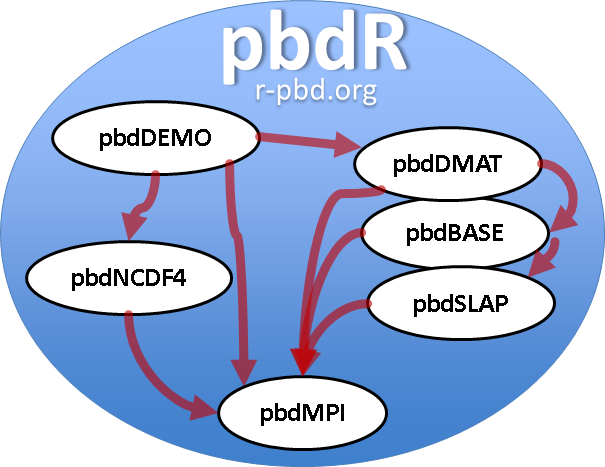
\includegraphics[scale=.4]{pics/pbdR}
        \end{column}
        \hfill
        \begin{column}{.4\textwidth}
      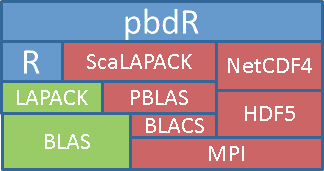
\includegraphics[scale=.45]{pics/libs}
        \end{column}
      \end{columns}
    \end{center}
  \end{block}
\end{frame}


\begin{frame}[fragile]
\begin{block}{pbdMPI vs Rmpi}
\pause
\begin{lstlisting}[title=Reduce Operation with Rmpi]
# int
mpi.allreduce(x, type=1)
# double
mpi.allreduce(x, type=2)
\end{lstlisting}

\begin{lstlisting}[title=Reduce Operation with pbdMPI]
allreduce(x)
\end{lstlisting}

\pause
\begin{lstlisting}
> is.integer(1)
[1] FALSE
> is.integer(2)
[1] FALSE
> is.integer(1:2)
[1] TRUE
\end{lstlisting}
\end{block}
\end{frame}


\begin{frame}
\begin{block}{pbdMPI vs Rmpi}
\begin{table}[h]
 \centering
 \caption{Runtimes (seconds) for $10,000 \times 10,000$ \code{allgather} with \pkg{Rmpi} and \pkg{pbdMPI}.}
 \label{tab:allgather}
 \begin{tabular}{rrrr}\hline\hline
  Cores & \pkg{Rmpi} & \pkg{pbdMPI} & Speedup \\\hline
  32    & 24.6       & 6.7          & 3.67 \\
  64    & 25.2       & 7.1          & 3.55 \\
  128   & 22.3       & 7.2          & 3.10 \\
  256   & 22.4       & 7.1          & 3.15 \\\hline\hline
 \end{tabular}
\end{table}
\end{block}
\end{frame}



\begin{frame}[fragile]
  \begin{block}{pbdR Example Syntax}
  \begin{lstlisting}
x <- x[-1, 2:5]
x <- log(abs(x) + 1)
xtx <- t(x) %*% x
ans <- svd(solve(xtx))
  \end{lstlisting}
  \begin{center}
  Look familiar?\\[.4cm]
  \emph{The above runs on 1 core with R or 10,000 cores with pbdR}
  \end{center}
  \end{block}
\end{frame}



%%% distributed:
% shared memory not enough, mkl, nautilus/kraken

%%% What is a supercomputer? (interconnect)

% \section{Supercomputers}

% \hidenum
% \begin{frame}[noframenumbering]
% \frametitle{Contents}
%  \tableofcontents[currentsection,hideallsubsections]
% \end{frame}
% \shownum



% \subsection{Supercomputing}

\begin{frame}
  \begin{block}{Shared and Distributed Memory Machines}
   \begin{center}
    \begin{minipage}{.475\textwidth}
    \begin{block}{Shared Memory}
     Direct access to read/change memory (one node)
      \begin{center}
      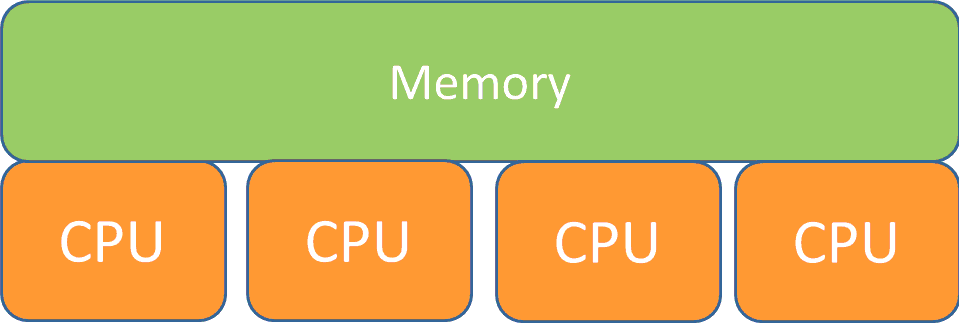
\includegraphics[width=.95\textwidth]{pics/arch_shared}
      \end{center}
      \vspace{.3cm} \
    \end{block}
    \end{minipage}
    \hspace{.1cm}
    \begin{minipage}{.475\textwidth}
    \begin{block}{Distributed}
    No direct access to read/change memory.
      \begin{center}
      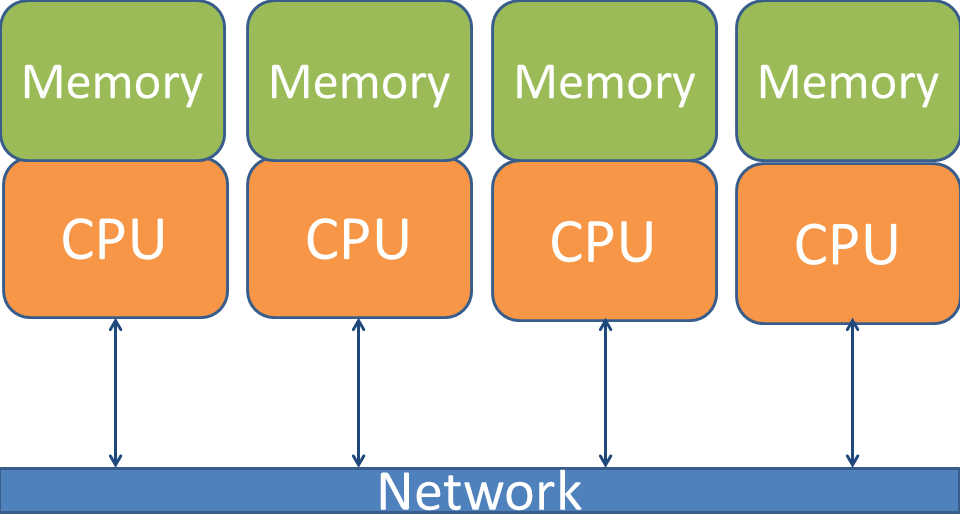
\includegraphics[width=.95\textwidth]{pics/arch_distributed}
      \end{center}
    \end{block}
    \end{minipage}
    \end{center}
    \end{block}
\end{frame}


\begin{frame}
  \begin{block}{Shared and Distributed Memory Machines}
   \begin{center}
    \begin{minipage}[t]{.47\textwidth}
    \begin{block}{Shared Memory Machines}
    \begin{center}
    Thousands of cores\\[.2cm]
    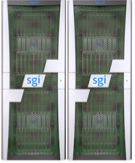
\includegraphics[scale=.65]{pics/nautilus}\\
    {\tiny \emph{Nautilus}, University of Tennessee\\1024 cores \\4 TB RAM\\}
    \end{center}
    \end{block}
    \end{minipage}
    \hspace{.1cm}
    \begin{minipage}[t]{.47\textwidth}
    \begin{block}{Distributed Memory Machines}
    \begin{center}
    Hundreds of thousands of cores\\[.2cm]
    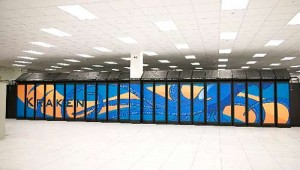
\includegraphics[width=.95\textwidth]{pics/kraken}\\
    {\tiny \emph{Kraken}, University of Tennessee\\ 112,896 cores \\147 TB RAM\\}
    \end{center}
    \end{block}
    \end{minipage}
    \end{center}
    \end{block}
\end{frame}



% \begin{frame}
% \frametitle{MKL Benchmark on $\approx 0.75$ GiB}
% \begin{center}
%     \hspace*{-1cm}\includegraphics[width=1.2\textwidth]{pics/rbenchmarkplotMatrix}  
% \end{center}
% \end{frame}


% \begin{frame}
%   \begin{block}{Terminology: Difficulty in Parallelism}
%     \begin{enumerate}[<+-|alert@+>]
%       \item \emph{Embarrassingly parallel}: easy/trivial to make parallel.
%       \item \emph{Tightly coupled}: difficult to make parallel.
%     \end{enumerate}
%   \end{block}
% \end{frame}




\section{Benchmarks}

\hidenum
\begin{frame}[noframenumbering]
\frametitle{Contents}
 \tableofcontents[currentsection,hideallsubsections]
\end{frame}
\shownum



\subsection{Benchmarks}

\begin{frame}
  \begin{block}{Non-Optimal Choices Throughout}
    \begin{enumerate}[<+-|alert@+>]
      \item Only libre software used (no MKL, ACML, etc.).
      \item 1 core = 1 MPI process.
      \item No tuning for data distribution.
    \end{enumerate}
  \end{block}
\end{frame}

\begin{frame}
  \begin{block}{Benchmark Data}
    \begin{enumerate}[<+-|alert@+>]
      \item Random normal $N(100, 10000)$.
      \item Local problem size of $\approx 43.4 MiB$.
      \item Three sets:  500, 1000, and 2000 columns.
      \item Several runs at different core sizes within each set.
    \end{enumerate}
  \end{block}
\end{frame}



% \subsection{Covariance}

\begin{frame}[fragile]
  \begin{block}{Covariance Code}
\begin{lstlisting}
x <- ddmatrix("rnorm", nrow=n, ncol=p, mean=mean, sd=sd)

cov.x <- cov(x)
\end{lstlisting}
  \end{block}
\end{frame}

\begin{frame}
  \begin{block}{\code{cov()}}
  \begin{center}
    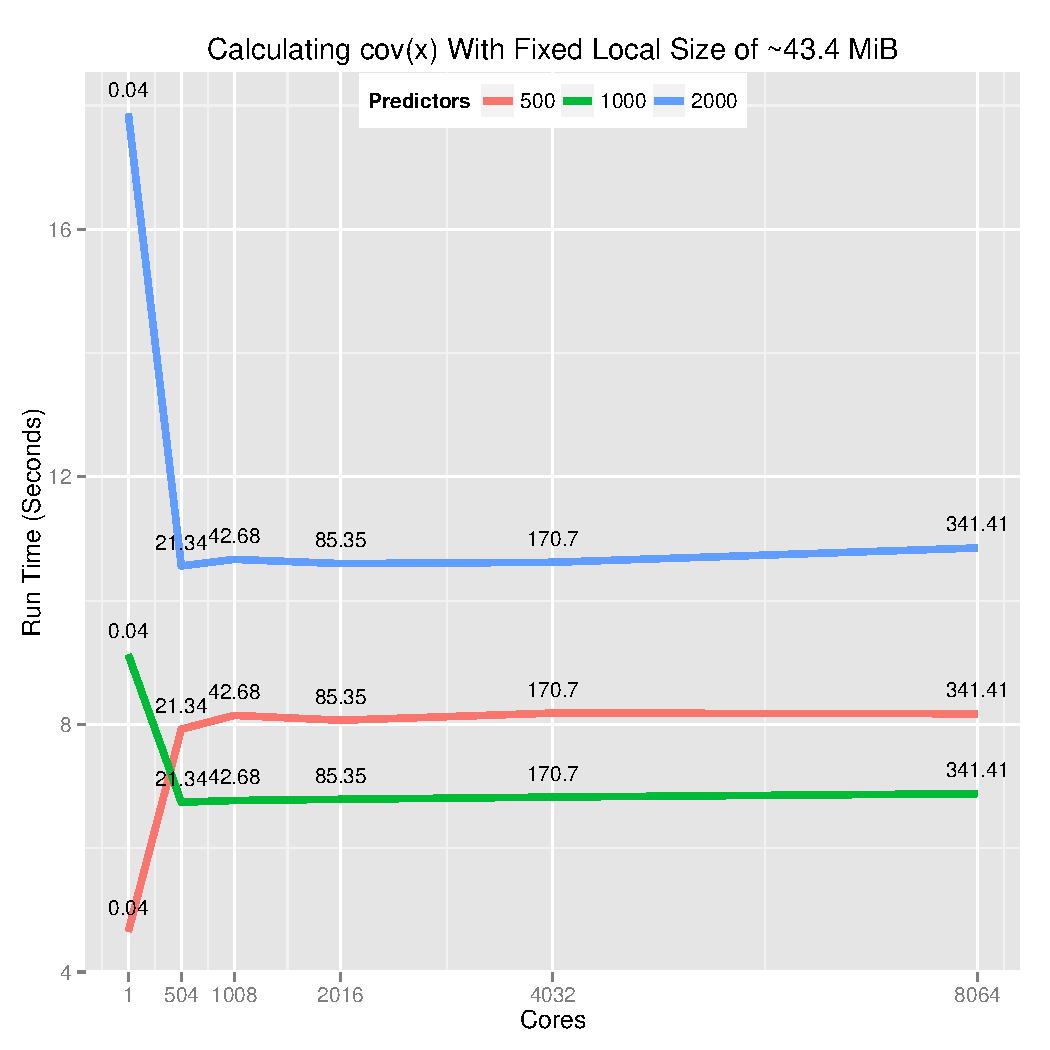
\includegraphics[height=.88\textheight]{pics/cov}
  \end{center}
  \end{block}
\end{frame}



% \subsection{Linear Model Fitting}

\begin{frame}[fragile]
  \begin{block}{Linear Model Code}
\begin{lstlisting}
x <- ddmatrix("rnorm", nrow=n, ncol=p, mean=mean, sd=sd)
beta_true <- ddmatrix("runif", nrow=p, ncol=1)

y <- x %*% beta_true

beta_est <- lm.fit(x=x, y=y)$coefficients
\end{lstlisting}
  \end{block}
\end{frame}

\begin{frame}
  \begin{block}{\code{Data Generation}}
  \begin{center}
    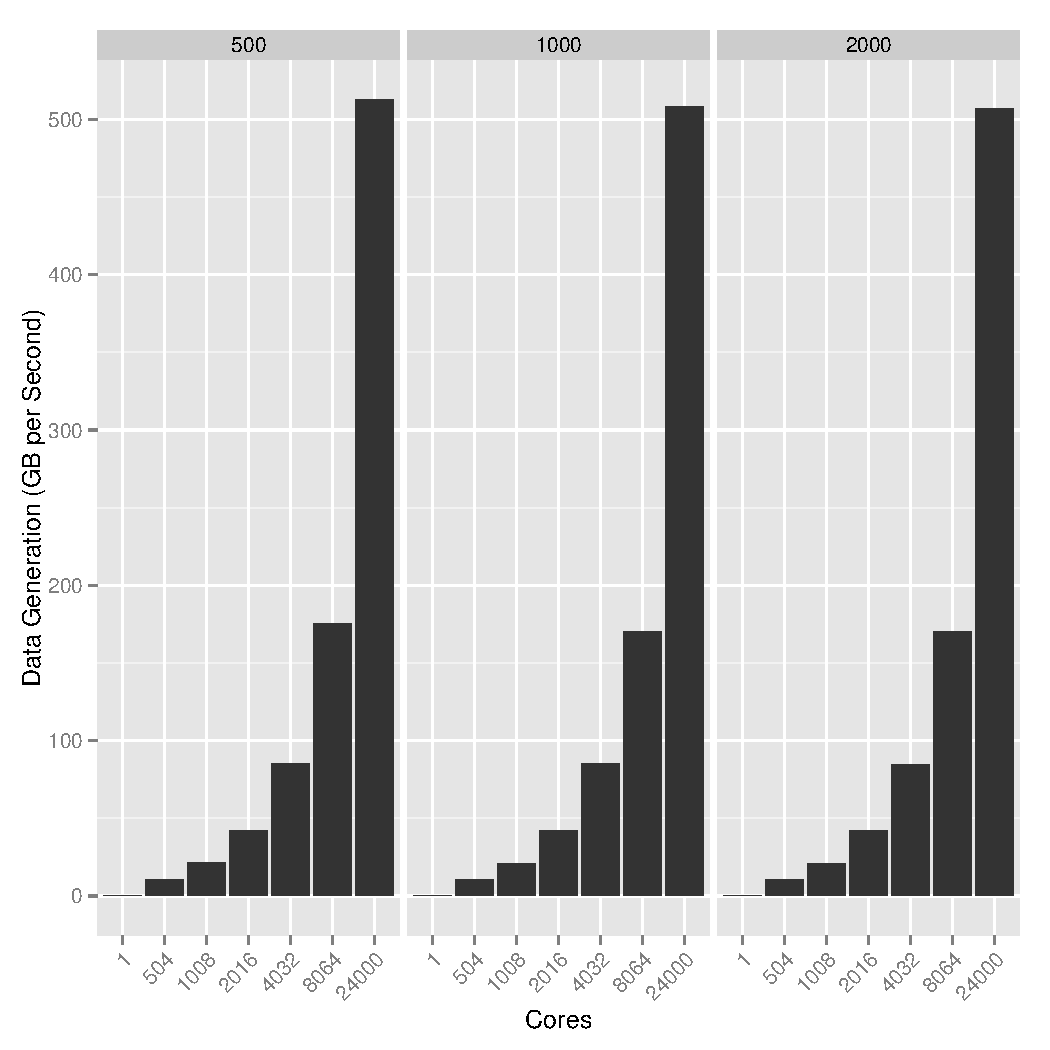
\includegraphics[height=.88\textheight]{pics/datagen}
  \end{center}
  \end{block}
\end{frame}

\begin{frame}
  \begin{block}{\code{lm.fit()}}
  \begin{center}
    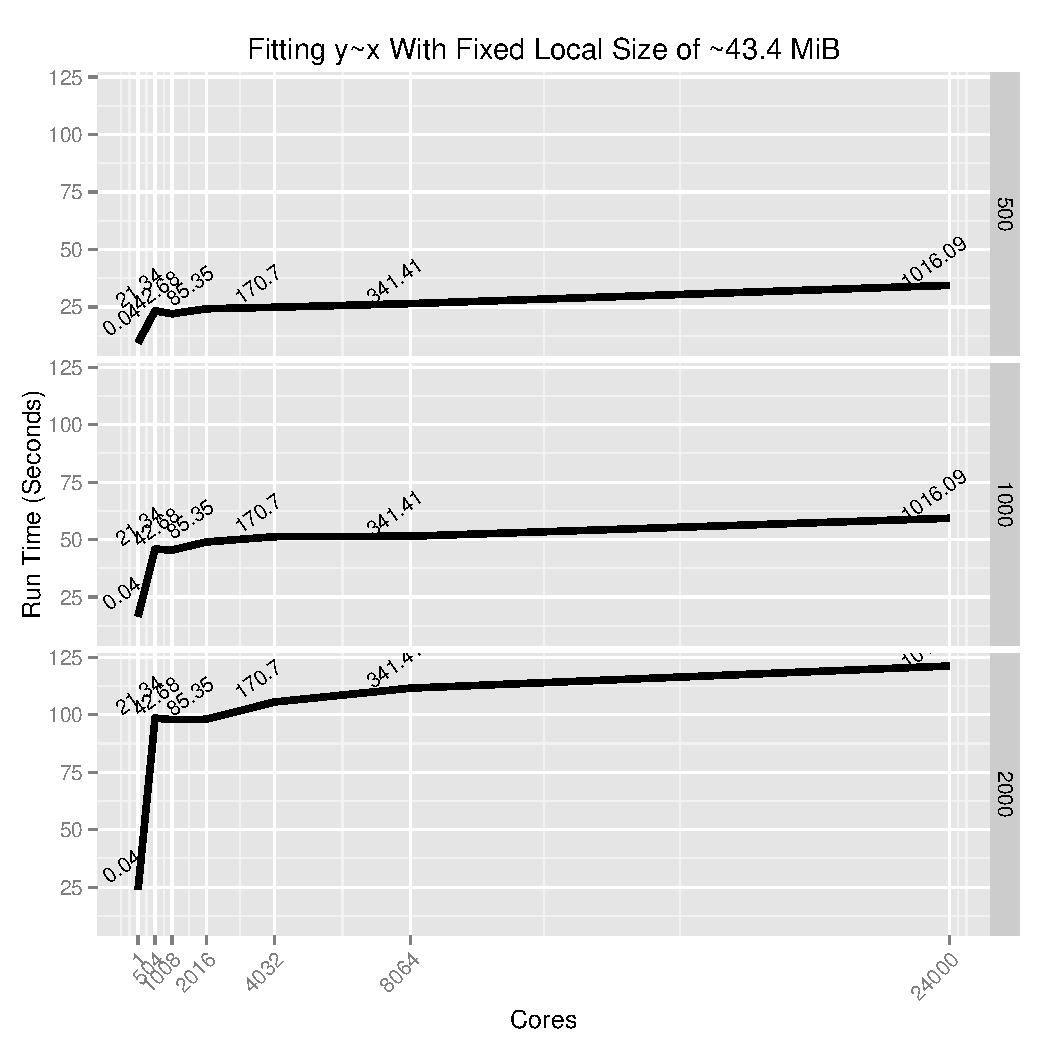
\includegraphics[height=.88\textheight]{pics/lmfit1}
  \end{center}
  \end{block}
\end{frame}

\begin{frame}
  \begin{block}{\code{lm.fit()}}
  \begin{center}
    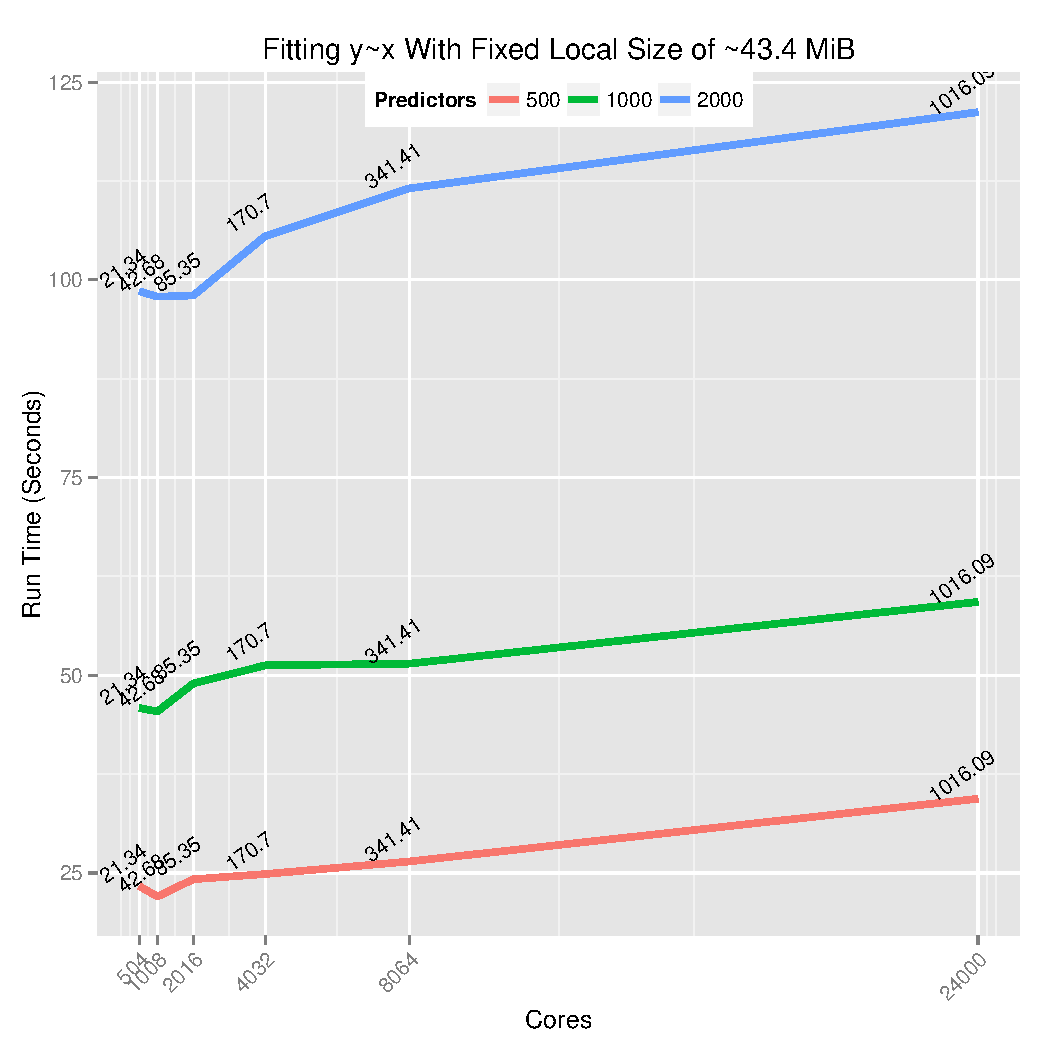
\includegraphics[height=.88\textheight]{pics/lmfit2}
  \end{center}
  \end{block}
\end{frame}
\section{Challenges}

\hidenum
\begin{frame}[noframenumbering]
\frametitle{Contents}
 \tableofcontents[currentsection,hideallsubsections]
\end{frame}
\shownum


\subsection{Challenges}

\begin{frame}
  \begin{block}{Challenges}
    \begin{itemize}[<+-|alert@+>]
      \item Perceptions.
      \item Library loading.
      \item Profiling.
    \end{itemize}
  \end{block}
\end{frame}


\begin{frame}
  \begin{block}{Covariance Revisited: Distributed Data Parameter Calibration}
    \begin{center}
     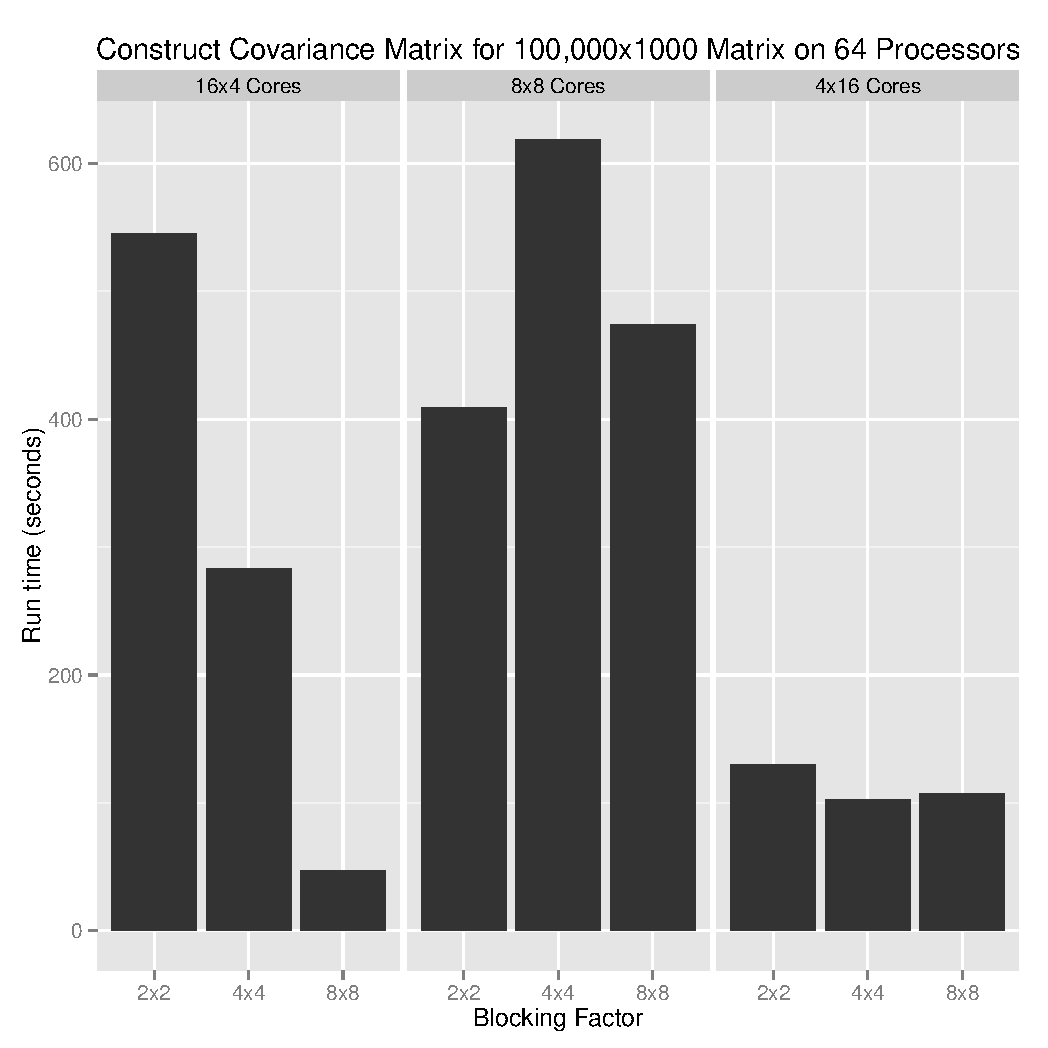
\includegraphics[width=10cm, height=7cm]{pics/cov_param}
    \end{center}
  \end{block}
\end{frame}

\begin{frame}
  \begin{block}{Tutorials}
  \begin{itemize}
    \item {\small XSEDE13, July 22, San Diego, California, USA }
    \item {\small SC13, November 17-22, Denver, Colorado, USA }
  \end{itemize}
  \end{block}
  \begin{block}{Invited Talks}
  \begin{itemize}
    \item {\small JSM 2013, August 3-8, Montr\'eal, Qu\'ebec }
    \item {\small IASC, Aug 22-23, Seoul}
    \item {\small World Statistics Congress, August 25-30, Hong Kong }
  \end{itemize}
  \end{block}
\end{frame}
  
\hidenum
\begin{frame}[noframenumbering]
 \begin{block}{Thanks for coming!}
 \begin{center}
     {\Large Questions?}\\[.6cm]
     \url{https://github.com/wrathematics/talks/blob/master/user2013/elevatingr.pdf?raw=true}
  \end{center}
 \end{block}
\end{frame}


\end{document}